\RequirePackage{luatex85}
\documentclass{standalone}

\usepackage{amsmath}
\newcommand{\vect}[1]{\mathbf{#1}}

\usepackage{fontspec, unicode-math}
\setsansfont[Scale=MatchLowercase]{TeX Gyre Heros}
\setmathfont{TeX Gyre Termes Math}

\usepackage{tikz}
%\usetikzlibrary{arrows.meta}
\usetikzlibrary{shapes}
\usepackage{pgfplots}
\pgfplotsset{compat=1.14}

\tikzset{
  every picture/.style={font={\sffamily\normalsize}, >=stealth},
  every pin edge/.style={black}}

\begin{document}

  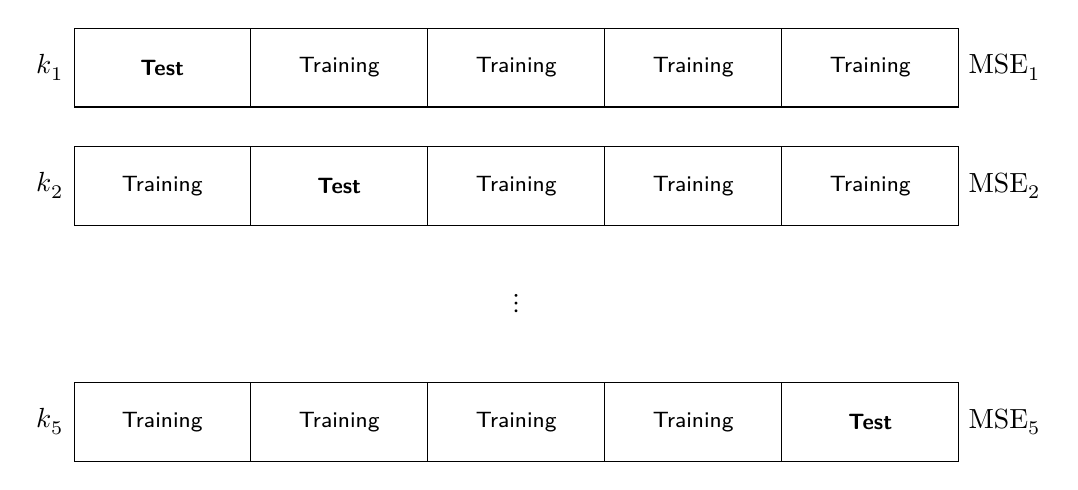
\begin{tikzpicture}[
    kFold/.style={
      draw, font=\sffamily\footnotesize,
      align=center,
      rectangle split,
      rectangle split horizontal,
      rectangle split parts=5,
      minimum height=1cm},
    fold/.style={text width=2cm}]

    \node[kFold] at (0, 10) [
           label=180:$k_{1}$,
           label=0:$\mathrm{MSE}_{1}$]
    {
      \nodepart[fold]{one}{\sffamily\bfseries Test}
      \nodepart[fold]{two}Training
      \nodepart[fold]{three}Training
      \nodepart[fold]{four}Training
      \nodepart[fold]{five}Training
    };
    
    \node[kFold] at (0, 8.5) [
           label=180:$k_{2}$,
           label=0:$\mathrm{MSE}_{2}$]
    {
      \nodepart[fold]{one}Training
      \nodepart[fold]{two}{\sffamily\bfseries Test}
      \nodepart[fold]{three}Training
      \nodepart[fold]{four}Training
      \nodepart[fold]{five}Training
    };

    \node at (0, 7) {$\vdots$};

    \node[kFold] at (0, 5.5) [
           label=180:$k_{5}$,
           label=0:$\mathrm{MSE}_{5}$]
    {
      \nodepart[fold]{one}Training
      \nodepart[fold]{two}Training
      \nodepart[fold]{three}Training
      \nodepart[fold]{four}Training
      \nodepart[fold]{five}{\sffamily\bfseries Test}
    };
  \end{tikzpicture}

\end{document}
